% Options for packages loaded elsewhere
\PassOptionsToPackage{unicode}{hyperref}
\PassOptionsToPackage{hyphens}{url}
\PassOptionsToPackage{dvipsnames,svgnames,x11names}{xcolor}
%
\documentclass[
  12pt]{article}

\usepackage{amsmath,amssymb}
\usepackage{iftex}
\ifPDFTeX
  \usepackage[T1]{fontenc}
  \usepackage[utf8]{inputenc}
  \usepackage{textcomp} % provide euro and other symbols
\else % if luatex or xetex
  \usepackage{unicode-math}
  \defaultfontfeatures{Scale=MatchLowercase}
  \defaultfontfeatures[\rmfamily]{Ligatures=TeX,Scale=1}
\fi
\usepackage{lmodern}
\ifPDFTeX\else  
    % xetex/luatex font selection
\fi
% Use upquote if available, for straight quotes in verbatim environments
\IfFileExists{upquote.sty}{\usepackage{upquote}}{}
\IfFileExists{microtype.sty}{% use microtype if available
  \usepackage[]{microtype}
  \UseMicrotypeSet[protrusion]{basicmath} % disable protrusion for tt fonts
}{}
\makeatletter
\@ifundefined{KOMAClassName}{% if non-KOMA class
  \IfFileExists{parskip.sty}{%
    \usepackage{parskip}
  }{% else
    \setlength{\parindent}{0pt}
    \setlength{\parskip}{6pt plus 2pt minus 1pt}}
}{% if KOMA class
  \KOMAoptions{parskip=half}}
\makeatother
\usepackage{xcolor}
\setlength{\emergencystretch}{3em} % prevent overfull lines
\setcounter{secnumdepth}{5}
% Make \paragraph and \subparagraph free-standing
\makeatletter
\ifx\paragraph\undefined\else
  \let\oldparagraph\paragraph
  \renewcommand{\paragraph}{
    \@ifstar
      \xxxParagraphStar
      \xxxParagraphNoStar
  }
  \newcommand{\xxxParagraphStar}[1]{\oldparagraph*{#1}\mbox{}}
  \newcommand{\xxxParagraphNoStar}[1]{\oldparagraph{#1}\mbox{}}
\fi
\ifx\subparagraph\undefined\else
  \let\oldsubparagraph\subparagraph
  \renewcommand{\subparagraph}{
    \@ifstar
      \xxxSubParagraphStar
      \xxxSubParagraphNoStar
  }
  \newcommand{\xxxSubParagraphStar}[1]{\oldsubparagraph*{#1}\mbox{}}
  \newcommand{\xxxSubParagraphNoStar}[1]{\oldsubparagraph{#1}\mbox{}}
\fi
\makeatother


\providecommand{\tightlist}{%
  \setlength{\itemsep}{0pt}\setlength{\parskip}{0pt}}\usepackage{longtable,booktabs,array}
\usepackage{calc} % for calculating minipage widths
% Correct order of tables after \paragraph or \subparagraph
\usepackage{etoolbox}
\makeatletter
\patchcmd\longtable{\par}{\if@noskipsec\mbox{}\fi\par}{}{}
\makeatother
% Allow footnotes in longtable head/foot
\IfFileExists{footnotehyper.sty}{\usepackage{footnotehyper}}{\usepackage{footnote}}
\makesavenoteenv{longtable}
\usepackage{graphicx}
\makeatletter
\def\maxwidth{\ifdim\Gin@nat@width>\linewidth\linewidth\else\Gin@nat@width\fi}
\def\maxheight{\ifdim\Gin@nat@height>\textheight\textheight\else\Gin@nat@height\fi}
\makeatother
% Scale images if necessary, so that they will not overflow the page
% margins by default, and it is still possible to overwrite the defaults
% using explicit options in \includegraphics[width, height, ...]{}
\setkeys{Gin}{width=\maxwidth,height=\maxheight,keepaspectratio}
% Set default figure placement to htbp
\makeatletter
\def\fps@figure{htbp}
\makeatother

\addtolength{\oddsidemargin}{-.5in}%
\addtolength{\evensidemargin}{-1in}%
\addtolength{\textwidth}{1in}%
\addtolength{\textheight}{1.7in}%
\addtolength{\topmargin}{-1in}%
\usepackage{booktabs}
\usepackage{longtable}
\usepackage{array}
\usepackage{multirow}
\usepackage{wrapfig}
\usepackage{float}
\usepackage{colortbl}
\usepackage{pdflscape}
\usepackage{tabu}
\usepackage{threeparttable}
\usepackage{threeparttablex}
\usepackage[normalem]{ulem}
\usepackage{makecell}
\usepackage{xcolor}
\makeatletter
\@ifpackageloaded{caption}{}{\usepackage{caption}}
\AtBeginDocument{%
\ifdefined\contentsname
  \renewcommand*\contentsname{Table of contents}
\else
  \newcommand\contentsname{Table of contents}
\fi
\ifdefined\listfigurename
  \renewcommand*\listfigurename{List of Figures}
\else
  \newcommand\listfigurename{List of Figures}
\fi
\ifdefined\listtablename
  \renewcommand*\listtablename{List of Tables}
\else
  \newcommand\listtablename{List of Tables}
\fi
\ifdefined\figurename
  \renewcommand*\figurename{Figure}
\else
  \newcommand\figurename{Figure}
\fi
\ifdefined\tablename
  \renewcommand*\tablename{Table}
\else
  \newcommand\tablename{Table}
\fi
}
\@ifpackageloaded{float}{}{\usepackage{float}}
\floatstyle{ruled}
\@ifundefined{c@chapter}{\newfloat{codelisting}{h}{lop}}{\newfloat{codelisting}{h}{lop}[chapter]}
\floatname{codelisting}{Listing}
\newcommand*\listoflistings{\listof{codelisting}{List of Listings}}
\makeatother
\makeatletter
\makeatother
\makeatletter
\@ifpackageloaded{caption}{}{\usepackage{caption}}
\@ifpackageloaded{subcaption}{}{\usepackage{subcaption}}
\makeatother

\ifLuaTeX
  \usepackage{selnolig}  % disable illegal ligatures
\fi
\usepackage[]{natbib}
\bibliographystyle{agsm}
\usepackage{bookmark}

\IfFileExists{xurl.sty}{\usepackage{xurl}}{} % add URL line breaks if available
\urlstyle{same} % disable monospaced font for URLs
\hypersetup{
  pdftitle={DOGE's Downsizing, Can AI Read the Reddit Room?},
  pdfauthor={Kevin Linares; Felix Baez-Santiago; Aria Lu; Gloria Zhou},
  colorlinks=true,
  linkcolor={blue},
  filecolor={Maroon},
  citecolor={Blue},
  urlcolor={Blue},
  pdfcreator={LaTeX via pandoc}}



\begin{document}


\def\spacingset#1{\renewcommand{\baselinestretch}%
{#1}\small\normalsize} \spacingset{1}


%%%%%%%%%%%%%%%%%%%%%%%%%%%%%%%%%%%%%%%%%%%%%%%%%%%%%%%%%%%%%%%%%%%%%%%%%%%%%%

\date{April 9, 2025}
\title{\bf DOGE's Downsizing, Can AI Read the Reddit Room?}
\author{
Kevin Linares\\
University of Maryland\\
and\\Felix Baez-Santiago\\
and\\Aria Lu\\
and\\Gloria Zhou\\
University of Michigan\\
}
\maketitle

\bigskip
\bigskip
\begin{abstract}
We investigated public sentiment on Reddit regarding the Department of
Government Efficiency's federal workforce reduction by classifying 400
labeled comments (28\% favor, 18\% neutral, 54\% oppose) using
supervised and unsupervised Large Language Models (LLMs). It turned out
that supervised models showed low to moderate success, particularly with
``oppose'' comments, but struggled with ``favor'' and ``neutral''
stances. Similarly, LLMs best intent identified ``oppose'' sentiment but
exhibited low precision for ``favor'' and ``neutral.'' These findings
highlight the challenges of accurately gauging nuanced public opinion on
government policy changes through automated methods on social media
data.
\end{abstract}


\newpage
\spacingset{1.9} % DON'T change the spacing!


\section{Introduction}\label{sec-intro}

The newly formed Department of Government Efficiency (DOGE) has reduced
the federal workforce by almost 280,000 employees, a central pledge of
the current administration. This action has generated significant
apprehension among federal workers in regards to mental health and job
security. To understand the impact of DOGE's actions on federal worker
perceptions of job security, we labeled 400 Reddit comments on topics
related to the current reduction in federal workforce by DOGE as whether
the author favored, opposed, or had a neutral stance. We use these
labels to build supervised learning models to predict stance.
Additionally, we employ unsupervised large language models (LLMs) to
detect the stance of these Reddit comments from text, to further explore
appropriate models for this current topic.

\section{Method}\label{sec-meth}

We collected a total of 12,553 Reddit comments in early March 2024 from
subreddits relevant to the topic of interest. These comments were
retrieved using keyword-based queries designed to capture posts of
discussions that would reflect users' stances on the federal workforce
reduction by DOGE. To prepare the data for analysis, a comprehensive
preprocessing pipeline was conducted in Python 3. This process involved
removing HTML tags and web-URLs, stripping special characters and
tagging artifacts such as ``@'', and replacing emojis with textual
descriptions. Also, it entailed eliminating punctuations and converting
numerical values into their spelled-out forms. The text was standardized
to lowercase, lemmatized using the SpaCy library, and further refined by
removing stopwords per the Natural Language Toolkit (NLTK) lists.
Spelling corrections were performed to improve textual coherence, while
duplicate comments were identified and removed to maintain data
integrity.

From this cleaned dataset, 400 unique comments without replacement were
randomly sampled for manual annotation. Four graduate students
independently coded and labeled each comment with one of three possible
stances: favor, oppose, or neutral toward DOGE's approach to federal
workforce reductions. As shown in Table 1, there were 28\% favor, 18\%
neutral, and 54\% oppose. These labeled comments were subsequently used
for training and evaluating both supervised and unsupervised
classification models.

\begin{longtable}[]{@{}cc@{}}
\caption{Distribution of Labeled Reddit Comment Data}\tabularnewline
\toprule\noalign{}
Stance & \% \\
\midrule\noalign{}
\endfirsthead
\toprule\noalign{}
Stance & \% \\
\midrule\noalign{}
\endhead
\bottomrule\noalign{}
\endlastfoot
favor & 27.5\% \\
neutral & 18.2\% \\
oppose & 54.2\% \\
\end{longtable}

The feature set used in model training and evaluation consisted of two
primary categories: metadata features and textual features. Metadata
features included the Reddit comment's score, the subreddit in which it
appeared in, and the search term that retrieved it. As the variables for
score and upvotes were perfectly collinear in this dataset, only the
score was retained. To ensure all values were non-negative, the score
was adjusted by subtracting the dataset's minimum value from each score.
The categorical variables, subreddit and search term, were numerically
encoded using scikit-learn's label encoder.

Textual features were derived from each comment and represented using
two distinct approaches: unigram term frequency and term
frequency-inverse document frequency (TF-IDF). The unigram used a
bag-of-words model to represent each word as a feature based on its
frequency in comment. The TF-IDF transformation built upon these raw
counts by accounting for term importance across the corpus. For both
unigram and TF-IDF methods, the total number of text-derived features
was 2,102. Combined with the three metadata features, each dataset
contained a total of 2,105 features. Two datasets were constructed for
classification: one combining the metadata with unigram features, and
another with metadata and TF-IDF features. Each dataset was divided into
80\% training data and 20\% test data. All supervised learning models
were implemented using Python 3, with scikit-learn and XGBoost as the
primary machine learning (ML) techniques. Classification was conducted
using a diverse set of algorithms, including Extra Trees Classifier,
Random Forest Classifier, Logistic Regression, Ridge Classifier,
K-Nearest Neightbors (KNN), Nearest Centroid, Multi-layer Perceptron
Classifier, Bernoulli Naive Bayes, Multino- mial Naive Bayes, Linear
Support Vector Classifier, Decision Tree Classifier, Extra Tree
Classifier, and the XGBoost Classifier.

All models were trained using default hyperparameter configurations. The
number of neighbors for KNN model was set to three, and the mtry
parameter for Random Forrest was fixed at two, reflecting the relatively
small number of metadata features in those models. All experiments were
conducted on a personal computer without the use of a GPU

In addition to traditional supervised models, we employed two
instruction-tuned LLMs to perform zero- shot classification: Gemma
3.12B, developed by Google and based on the Gemini framework, and LLaMA
3.2B, developed by Meta AI. Gemma was deployed using the Great Lakes
High-Performance Computing (HPC) cluster, while LLaMA was deployed
locally on a GPU-enabled personal workstation using the rollama
r-pacakge. These models were selected for their strong zero-shot
classification capabilities and ability to be run locally or on cluster
environments without reliance on commercial APIs. Both models were given
the same prompt and tasks, which were developed by the research team to
assess the effectiveness of classifying stance within our topic of
interest (see Table 2).

\hfill\break

Table 2. Example of Prompt and Task for LLMs

\begin{longtable}[]{@{}
  >{\raggedright\arraybackslash}p{(\columnwidth - 2\tabcolsep) * \real{0.2778}}
  >{\raggedright\arraybackslash}p{(\columnwidth - 2\tabcolsep) * \real{0.7222}}@{}}
\toprule\noalign{}
\endhead
\bottomrule\noalign{}
\endlastfoot
\textbf{Prompt}: & ``Is this comment in `favor', `neutral', or `oppose'
the reduction in federal workforce? Provide one word answer only! \\
\textbf{Task}: & ``You have assumed the role of a stakeholder that is
presented with a Reddit comment from a likely federal worker related to
the current policies on reducing the federal workforce. Please determine
the author's stance on this topic, and provide the answer only.'' \\
\end{longtable}

The model performance was evaluated by the F1-score and recall. The
F1-score, a harmonic mean of precision and recall, serves as a balanced
indicator of a model's ability to correctly identify relevant instances
while minimizing both false positives and false negatives. Recall was
also independently assessed to evaluate the proportion of true positive
cases accurately identified by each model. While a high recall may
increase the risk of false positives, its combination with the F1-score
allows a more robust evaluation of model performance, especially for
addressing the challenges inherent in imbalanced classification tasks

\section{Results}\label{results}

Our machine learning models revealed a mix of performance results in
classifying the stance of Reddit comment into ``favor'', ``neutral'',
and ``oppose.'' Both models exhibited low recall and F1-scores for the
``favor'' stance (see Figure 1), and the random forest model (recall
.26: F1-score .28) slightly outperformed KNN (recall .16: F1-score .19).
The ``neutral'' class presented a significant challenge for the random
forest with very low scores (recall .05: F1-score .10), while KNN
exhibited slightly better performance (recall .21: F1-score .21). Both
models showed the strongest performance in identifying comments
expressing opposition. The random forest correctly identified 74\% of
all the actual Reddit comments expressing opposition compared to KNN at
64\%, suggesting that KNN missed a larger proportion of true ``oppose''
comments. Both models obtained similar F!- scores of 60\%, suggesting
that KNN may have slightly higher precision, given its lower recall
compared to the random forest model. This implies that when KNN predicts
comments for the ``oppose'' class, its accuracy is comparable to that of
the random forest model.

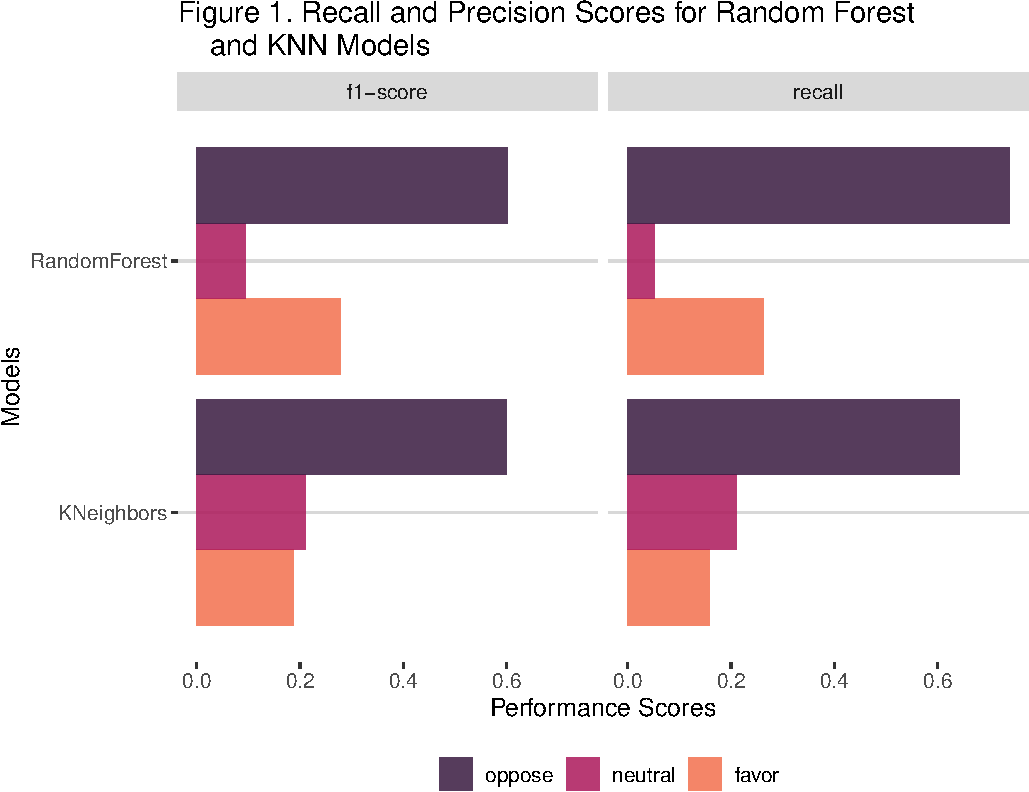
\includegraphics{assign_3_files/figure-pdf/unnamed-chunk-3-1.pdf}

The LLMs, showed poor performance in classifying the ``favor'' stance,
with very low F1-scores (Llama .07: Gemma .02) despite moderate recall
(Llama .29: Gemma .33), indicating low precision (see Figure 2). For the
``neutral'' class, both models showed modest results, with Llama
achieving a slightly better F1-score (.23) compared to Gemma (.18),
although Gemma had a higher recall (Gemma .50: Llama .25), again
suggesting lower precision for Gemma. Similar to the supervised models,
both LLMs performed best in classifying the ``oppose'' stance, with
relatively high and similar F1-scores (Llama .67: Gemma .70) and
comparable recall (Llama .56: Gemma .56), suggesting a better balance
between precision and recall for this category. Both models correctly
identified 67\% to 70\% of all the actual Reddit comments expressing
opposition. Overall, both LLMs struggled with the ``favor'' and
``neutral'' stance but demonstrated a stronger ability to identify
opposing comments.\\

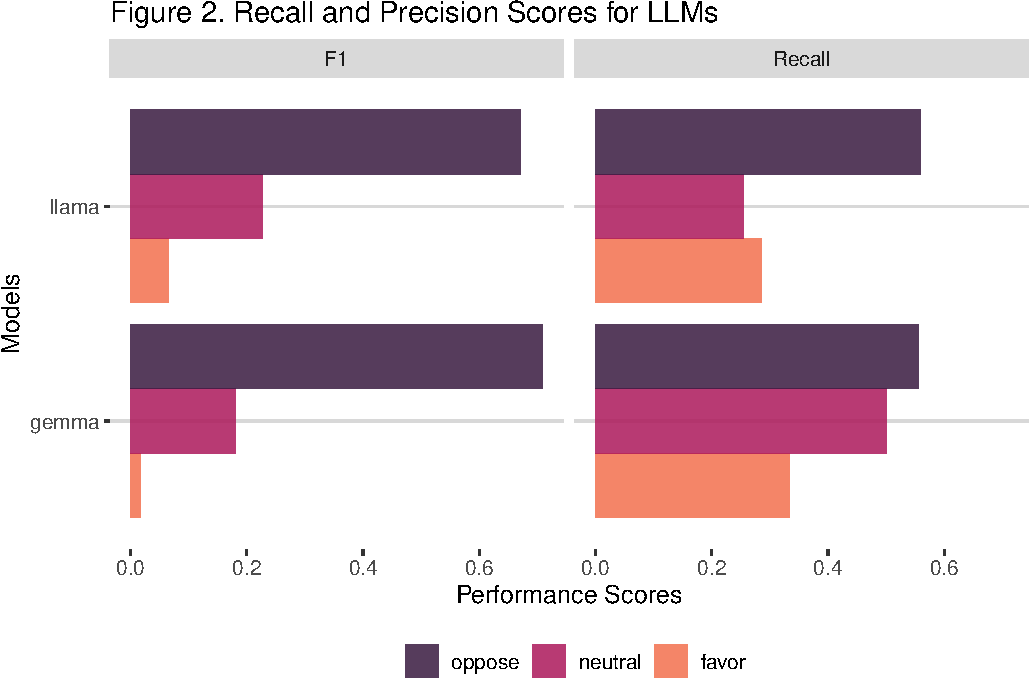
\includegraphics{assign_3_files/figure-pdf/unnamed-chunk-5-1.pdf}

Gemma and Llama demonstrated only fair agreement in stance
classification (Cohen's Kappa = .24). The contingency table ( see Table
3) reveals the highest agreement for ``oppose'' (.80), indicating some
consistency in identifying a strong negative stance. However, agreement
was substantially lower for ``neutral'' (.03) and ``favor'' (.01),
highlighting the divergent interpretations of more nuanced language. The
off-diagonal values further illustrates these discrepancies, suggesting
the fundamental differences in how the models process ambiguous cues and
establish classification boundaries, particularly for less extreme
stances.

\begin{longtable}[]{@{}lrrr@{}}
\caption{Aggreement Between LLMs, Cohen's Kappa, 0.24}\tabularnewline
\toprule\noalign{}
& favor & neutral & oppose \\
\midrule\noalign{}
\endfirsthead
\toprule\noalign{}
& favor & neutral & oppose \\
\midrule\noalign{}
\endhead
\bottomrule\noalign{}
\endlastfoot
favor & 3 & 1 & 10 \\
neutral & 0 & 10 & 49 \\
oppose & 0 & 5 & 317 \\
\end{longtable}

\section{Conclusion}\label{conclusion}

Public sentiment on Reddit were explored in terms of the DOGE federal
workforce reduction through supervised learning (KNN, Random Forest) and
unsupervised LLMs ( Gemma 3.12b and Llama 3.2 3B) for stance
classifications. Our supervised learning models overall achieved low to
moderate success in this classification task, with the strongest
performance in identifying opposing viewpoints, which were also the most
prevalent in our labeled data. Moreover, both models struggled with the
``favor'' and ``neutral'' stances, suggesting limitations in our
features to capture these nuances. Our unsupervised learning models also
showed the best ability to classify ``oppose'' comments, yet exhibited
significant challenges with the ``favor'' and ``neutral'' categories,
particularly demonstrating low precision.

This study had limitations such as the small size of our labelled
dataset of 400 Reddit comments, the imbalance in the stance categories,
and few features in the supervised approach. The zero-shot capabilities
of the LLMs are suitable for topic exploration but may require
fine-tuning for optimal performance on this specific domain,
particularly with nuance language used in ``favor'' stance. To deepen
the understanding of federal worker perceptions and enhance stance
classification, future research may further expand the labeled datasets
and incorporate more contextual text, rather than relying on single
comments. Fine tuning LLMs on a larger corpus with relevant comments
could render more accuracy in the classification task.




\end{document}
